\documentclass[11pt]{dinbrief}
\usepackage[T1]{fontenc}
\usepackage[utf8]{inputenc}
\usepackage[ngerman]{babel}
\usepackage[babel,german=quotes]{csquotes} % Für gute Anführungszeichen
\usepackage{lmodern}
\usepackage{graphicx}

%\textwidth12cm

\setaddresswidth{75mm}
\setaddressheight{40mm}
\setaddressllcorner{25mm}{90mm}
\setbottomtexttop{270mm}  % x from top of page
\bottomtext{\kern27mm%    % y from bottom of page; x+y=297mm
    \vbox to 0pt{\vss\hbox to 0pt{\kern-2.5cm
    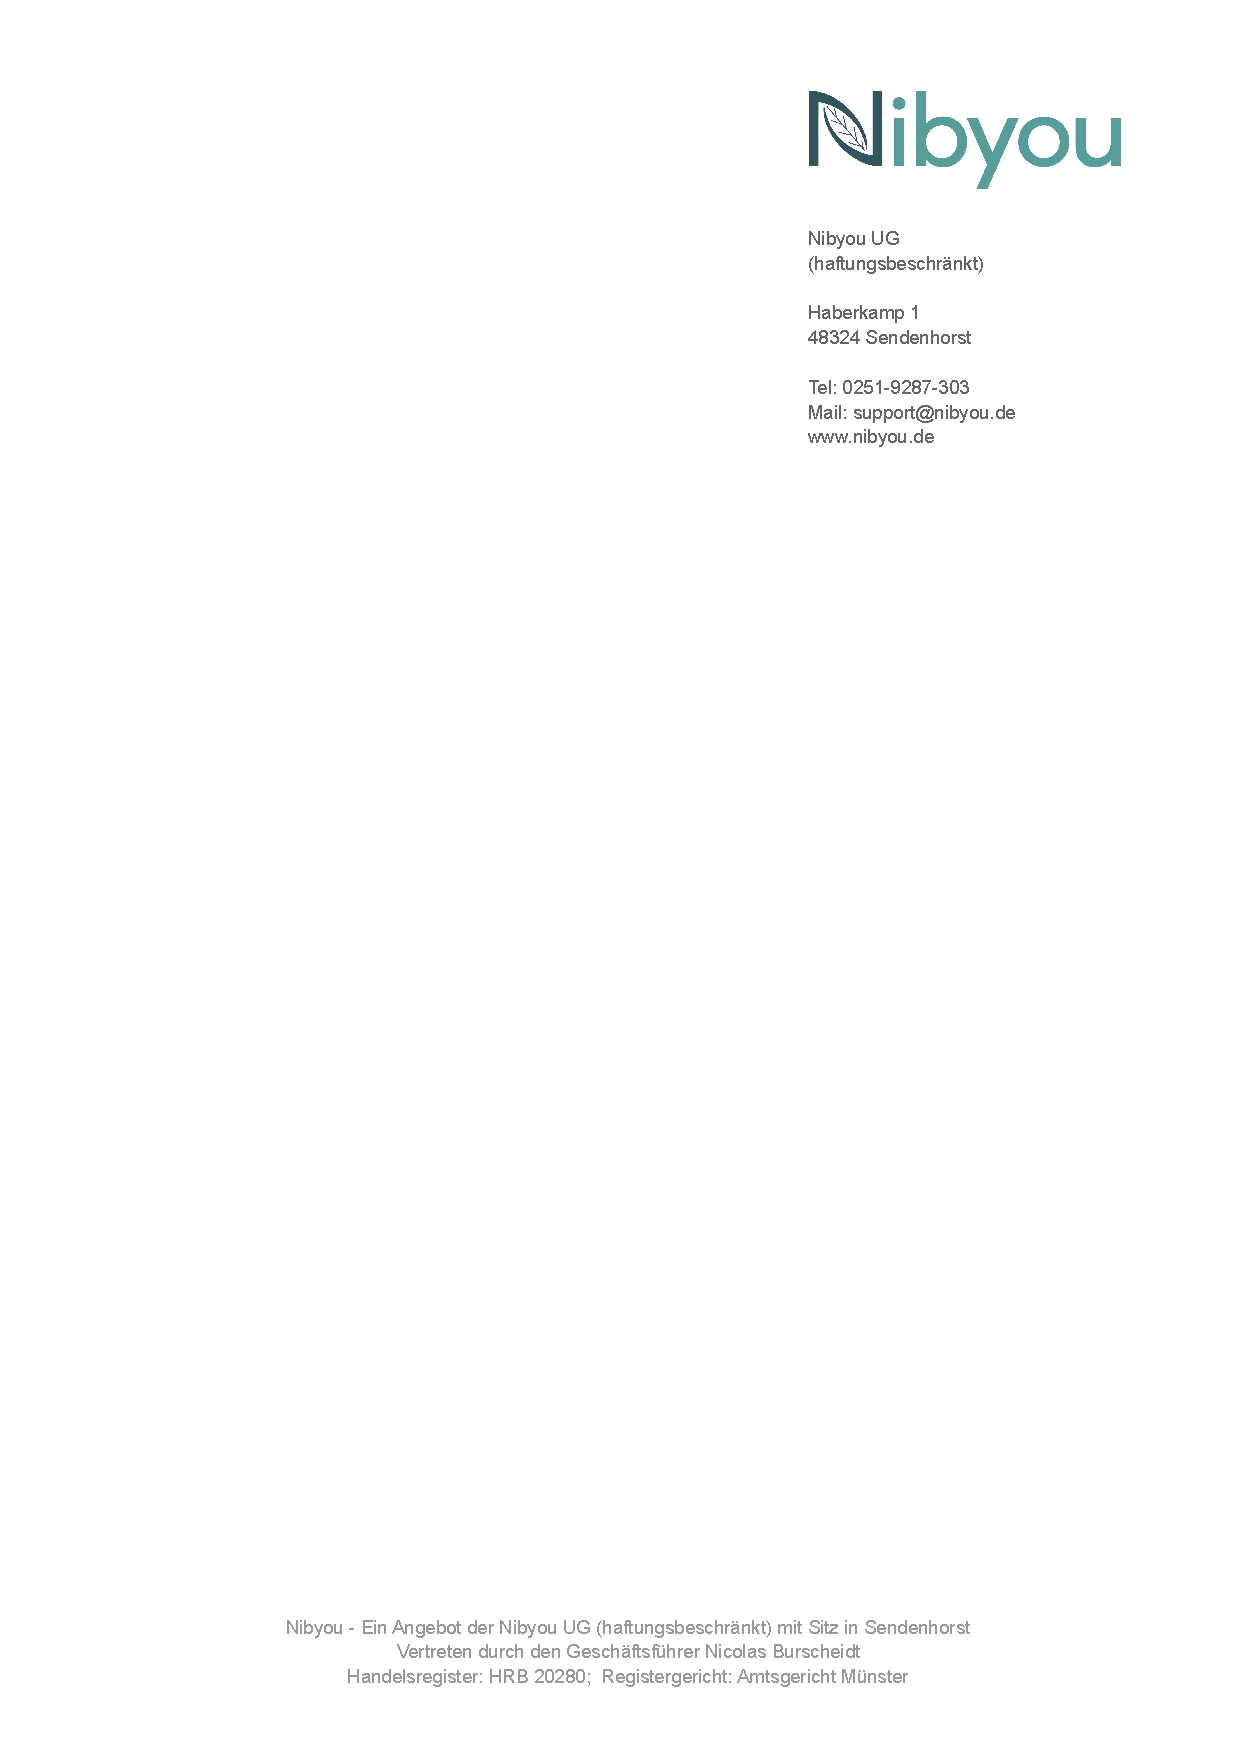
\includegraphics{letterhead.pdf}\hss}}}

\begin{document}
\centeraddress
\backaddress{Nibyou UG $\cdot$ Haberkamp 1 $\cdot$ 48324 Sendenhorst}
%\nobackaddressrule
\signature{Ihr Nibyou Team}
\place{Sendenhorst}
\date{\today}
\begin{letter}{ {{toAddress}} }
  \nowindowrules
  \nowindowtics
\opening{ {\Large \textbf{Ihr persöhnliches Recovery-Passwort} } \\ \ \\Guten Tag {{name}},}
wir freuen uns Ihnen heute Ihr neues persönliches Recovery-Passwort zuzusenden. Mit diesem können Sie in Zukunft bei Passwort-Verlust Ihr Passwort zurücksetzen. \\ \ \\
Ihr Recovery-Passwort lautet:\\
\textbf{ {{recoveryPassword}} }
\\ \ \\
Bewahren Sie das Recovery-Passwort unbedingt sicher auf. Bei Verlust von Passwort und Recovery-Passwort, verlieren Sie den Zugang zu Ihren Patientendaten unwiderruflich. \\ \ \\
Für Fragen stehen wir Ihnen gerne zur Verfügung.
\closing[]{Mit freundlichen Grüßen aus dem Münsterland,}
\end{letter}
\end{document}
